\subsection{Riemann-Liouville Integral}\label{sec:RL}
The Riemann-Liouville integral of order $\alpha$ is defined as
\begin{equation}
    J^\alpha y(t) = \dfrac{1}{\Gamma(\alpha)}\int_{0}^{t}\dfrac{y(\lambda)}{(t-\lambda)^{1-\alpha}}d\lambda
\end{equation}

\begin{theorem}
Let $\alpha,\beta\in\mathbb{R}^+$, then
\begin{equation}
    J^\alpha J^\beta y(t) = J^{\alpha+\beta} y(t)
\end{equation}
\end{theorem}
\begin{proof}
\begin{align*}
    J^{\alpha}J^{\beta}y(t)&=\dfrac{1}{\Gamma(\alpha)} \int_0^t\dfrac{\left(J^{\beta}y(t)\right)(\lambda_1)}{(t-\lambda_1)^{1-\alpha}}d\lambda_1\\
    &=\dfrac{1}{\Gamma(\alpha)} \int_0^t\dfrac{1}{(t-\lambda_1)^{1-\alpha}\Gamma(\beta)}\int_0^{\lambda_1}\dfrac{y(\lambda_2)}{(\lambda_1-\lambda_2)^{1-\beta}}d\lambda_2d\lambda_1\\
    &=\dfrac{1}{\Gamma(\alpha)\Gamma(\beta)}\int_0^{t}\int_0^{\lambda_1}(t-\lambda_1^{\beta-1})(\lambda_1-\lambda_2)^{\alpha-1}y(\lambda_2)d\lambda_2d\lambda_1\\
    &=\dfrac{1}{\Gamma(\alpha)\Gamma(\beta)}\int_0^{t}\int_{\lambda_2}^t (t-\lambda_1^{\beta-1})(\lambda_1-\lambda_2)^{\alpha-1}y(\lambda_2)d\lambda_1d\lambda_2\\
    &=\dfrac{1}{\Gamma(\alpha)\Gamma(\beta)}\int_0^{t}y(\lambda_2)\int_{\lambda_2}^t(t-\lambda_1^{\beta-1})(\lambda_1-\lambda_2)^{\alpha-1}y(\lambda_2)d\lambda_1d\lambda_2\\
\end{align*}
Multiplying and dividing by $(t-\lambda_2)^{\alpha+\beta-2}$
\begin{align*}
    J^{\alpha}J^{\beta}y(t)&=\dfrac{1}{\Gamma(\alpha)\Gamma(\beta)}\int_0^{t}(t-\lambda_2)^{\alpha+\beta-2}y(t_2)\int_{\lambda_2}^{t}\left(\dfrac{t-\lambda_1}{t-\lambda_2}\right)^{\beta-1}\left(\dfrac{\lambda_1-\lambda_2}{t-\lambda_2}\right)^{\alpha-1}d\lambda_1d\lambda_2
\end{align*}
Let $u=\dfrac{\lambda_1-\lambda_2}{t-\lambda_2}\rightarrow du=\dfrac{d\lambda_1}{t-\lambda_2}$. Note that $1-u=\dfrac{t-\lambda_1}{t-\lambda_2}$
\begin{align*}
    J^{\alpha}J^{\beta}y(t)&=\dfrac{1}{\Gamma(\alpha)\Gamma(\beta)}\int_0^{t}(t-\lambda_2)^{\alpha+\beta-2}y(t_2)\int_0^1\dfrac{u^{\beta-1}(1-u)^{\alpha-1}}{t-\lambda_2}dud\lambda_2\\
    &=\dfrac{1}{\Gamma(\alpha)\Gamma(\beta)}\int_0^{t}(t-\lambda_2)^{\alpha+\beta-1}y(t_2)B(\beta,\alpha)d\lambda_2\\
    &=\dfrac{1}{\Gamma(\alpha+\beta)}\int_0^{t}(t-\lambda_2)^{\alpha+\beta-1}y(t_2)d\lambda_2=J^{\alpha+\beta}y(t)
\end{align*}
\end{proof}



\section{Caputo Fractional Derivative}

The $\alpha$-order Caputo derivative is defined as 
\begin{equation}
    \mathcal{D}_c^\alpha y(t) = J^{m-\alpha}y^{(m)}(t) = \dfrac{1}{\Gamma(m-\alpha)}\int_0^t \dfrac{y^{(m)}(\lambda)}{(t-\lambda)^{1-m+\alpha}}d\lambda
\end{equation}

Where $m = \ceil{\alpha}$. We assume $\alpha\geq0$. Note that some authors, e.g. \cite{kisela2008fractional}, treat $\alpha<0$ as a fractional integral. 

The main feature of the Caputo definition is that, when defining a fractional differential equation (FDE) involving this definition, they only require initial conditions for the derivatives of integer order, unlike Riemann-Liouville definition. This opens the FDEs to have an easier physical interpretation and modeling real systems.
\begin{exmp}
    Evaluate $\mathcal{D}_c^{0.5}\,t$
    \begin{align*}
      \mathcal{D}_c^{0.5}\,t &= \dfrac{1}{\Gamma(1-0.5)}\int_0^t \dfrac{d}{d\lambda}(\lambda)\cdot\dfrac{d\lambda}{(t-\lambda)^{1-0.5+1}}\\
      &= \dfrac{1}{\sqrt{\pi}}\int_0^t \dfrac{d\lambda}{(t-\lambda)^{1/2}}\quad\text{, let $u=t-\lambda$ $\rightarrow$ $du=-d\lambda$.}\\
      &= \dfrac{1}{\sqrt{\pi}}\int_0^t \dfrac{du}{u^{1/2}}\\
      &=2\sqrt{\dfrac{t}{\pi}}
    \end{align*}
\end{exmp}
    In order to illustrate the fractional derivative, we present the Caputo derivative of $y(t)=t$ for different orders in figure \ref{fig:t_derivative}. It can be proved that the Caputo-type derivative converges to the standard derivative for integer orders \cite{ishteva2005properties}, as depicted in this figure.
    
    \begin{figure}[H]
        \centering
        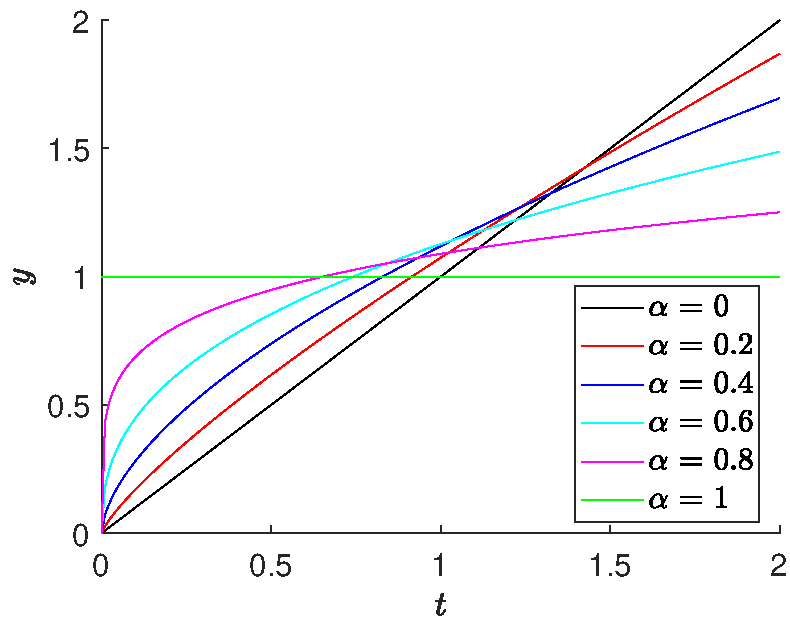
\includegraphics[scale=.5]{files/t_derivative.pdf}
        \caption{Fractional derivatives of $y(t)=t$ for different orders.}
        \label{fig:t_derivative}
    \end{figure}
    
    \begin{exmp}
        Evaluate $\mathcal{D}_c^\alpha\,t^r$
        \begin{align*}
        \mathcal{D}_c^\alpha\,t^r &= \dfrac{1}{\Gamma(m-\alpha)} \int_0^t \dfrac{d^m}{d\lambda^m}(\lambda^r)\cdot\dfrac{d\lambda}{(t-\lambda)^{1-m+\alpha}}\\
        & = \dfrac{1}{\Gamma(m-\alpha)}\int_0^t \dfrac{\Gamma(r+1)}{\Gamma(r-m+1)}\lambda^{r-m}\cdot\dfrac{d\lambda}{(t-\lambda)^{1-m+\alpha}}\\
        &= \dfrac{\Gamma(r+1)}{\Gamma(m-\alpha)\Gamma(r-m+1)}\int_0^t \lambda^{r-m}(t-\lambda)^{m-\alpha-1}d\lambda
    \end{align*}
    \end{exmp}
    Let $\lambda = u t$ $\rightarrow$ $d\lambda=tdu$. Note that $0\leq u\leq 1$.
    \begin{align*}
        \mathcal{D}_c^\alpha\,t^r &= \dfrac{\Gamma(r+1)}{\Gamma(m-\alpha)\Gamma(r-m+1)}\int_0^1 (u t)^{r-m}(t-u t)^{m-\alpha-1}tdu\\
        &=\dfrac{\Gamma(r+1)}{\Gamma(m-\alpha)\Gamma(r-m+1)}t^{r-\alpha}\int_0^1 u^{(r-m+1)-1}(1-u)^{(m-\alpha)-1}du\\
        &=\dfrac{\Gamma(r+1)}{\Gamma(m-\alpha)\Gamma(r-m+1)}t^{r-\alpha}\cdot B(r-m+1,m-\alpha)\\
        &=\dfrac{\Gamma(r+1)}{\Gamma(m-\alpha)\Gamma(r-m+1)}t^{r-\alpha}\cdot\dfrac{\Gamma(r-m+1)\Gamma(m-\alpha)}{\Gamma(r-\alpha+1)}\\
        &= \dfrac{\Gamma(r+1)}{\Gamma(r-\alpha+1)}t^{r-\alpha}\\
    \end{align*}
    
    \begin{theorem}\label{theo:leftinverse}
        $\mathcal{D}_c^\alpha$ is a left-inverse operator for $J^\alpha$.
    \end{theorem}
    \begin{proof}
        \begin{equation}
    \mathcal{D}_c^\alpha J^\alpha y(t) = J^{m-\alpha}\underset{\Delta}{\underbrace{\left(\dfrac{d^m}{dt^m}J^\alpha y(t)\right)}}
\end{equation}\label{eq:Jinverse}
Let us work on $\Delta$ first,

\begin{align*}
    \Delta&=\dfrac{d^m}{dt^m}\left[\dfrac{1}{\Gamma(\alpha)}\int_0^t\dfrac{y(\lambda_1)d\lambda_1}{(t-\lambda_1)^{1-\alpha}}\right]\\
    &= \dfrac{1}{\Gamma(\alpha)}\left[\dfrac{d^m}{dt^m}\int_0^t\dfrac{y(\lambda_1)d\lambda_1}{(t-\lambda_1)^{1-\alpha}}\right]\\
\end{align*}

Recall the Leibniz rule
\begin{equation}
    \dfrac{d}{dx}\int_{a(x)}^{b(x)}f(x,t)dt = f(x,b(x))\dfrac{db(x)}{dx}-f(x,a(x))\dfrac{da(x)}{dx}+\int_{a(x)}^{b(x)}\dfrac{\partial f(x,t)}{\partial x}dt
\end{equation}

Therefore,
\begin{align*}
    =\dfrac{d^{m-1}}{dt^{m-1}}\left[(t-t)^{\alpha-1}y(t) - 0 + \int_{0}^t \dfrac{(\alpha-1)y(\lambda_1)d\lambda_1}{(t-\lambda_1)^{2-\alpha}}\right]
\end{align*}

Applying this process recursively,
\begin{align*}
    =\dfrac{\Gamma(\alpha)}{\Gamma(\alpha-m)}\int_0^t\dfrac{y(\lambda_1)d\lambda_1}{(t-\lambda_1)^{1+m-\alpha}}
\end{align*}

Replacing in equation \eqref{eq:Jinverse},
\begin{align*}
    J^{m-\alpha}\left(\dfrac{d^m}{dt^m}J^\alpha y(t)\right)=&\dfrac{1}{\Gamma(\alpha-m)\Gamma{(m-\alpha)}}\int_0^t \dfrac{1}{(t-\lambda_2)^{1+\alpha-m}}\int_0^{\lambda_2} \dfrac{y(\lambda_1)d\lambda_1d\lambda_2}{(\lambda_2-\lambda_1)^{1-\alpha+m}}\\
    =& \dfrac{1}{\Gamma(\alpha-m)\Gamma{(m-\alpha)}}\int_0^t\int_0^{\lambda_2}  \dfrac{y(\lambda_1)d\lambda_1d\lambda_2}{(t-\lambda_2)^{1+\alpha-m}(\lambda_2-\lambda_1)^{1-\alpha+m}}\\
    =& \dfrac{1}{\Gamma(\alpha-m)\Gamma{(m-\alpha)}}\int_0^t\int_{\lambda_1}^{t}
    \dfrac{y(\lambda_1)d\lambda_2d\lambda_1}{(t-\lambda_2)^{1+\alpha-m}(\lambda_2-\lambda_1)^{1-\alpha+m}}\\
    =& \dfrac{1}{\Gamma(\alpha-m)\Gamma{(m-\alpha)}}\int_0^ty(\lambda_1)\int_{\lambda_1}^{t}
    \dfrac{d\lambda_2d\lambda_1}{(t-\lambda_2)^{1+\alpha-m}(\lambda_2-\lambda_1)^{1-\alpha+m}}
\end{align*}
Multiplying and dividing by $(t-\lambda_1)^{-2}$ yields

\begin{align*}
    J^{m-\alpha}\left(\dfrac{d^m}{dt^m}J^\alpha y(t)\right)=& \dfrac{1}{\Gamma(\alpha-m)\Gamma{(m-\alpha)}}\int_0^t(t-\lambda_1)^{-2}y(\lambda_1)\int_{\lambda_1}^{t} \psi(t,\lambda_1,\lambda_2,\alpha,m)d\lambda_2d\lambda_1
\end{align*}
where
\begin{equation*}
\psi(t,\lambda_1,\lambda_2,\alpha,m)=\left(\dfrac{t-\lambda_2}{t-\lambda_1}\right)^{m-\alpha-1}\left(\dfrac{\lambda_2-\lambda_1}{t-\lambda_1}\right)^{\alpha-1-m}
\end{equation*}


Let $u=\dfrac{\lambda_2-\lambda_1}{t-\lambda_1}\rightarrow du=\dfrac{d\lambda_2}{t-\lambda_1}$. Note that $1-u=\dfrac{t-\lambda_2}{t-\lambda_1}$, thus

\begin{align*}
    J^{m-\alpha}\left(\dfrac{d^m}{dt^m}J^\alpha y(t)\right)=& \dfrac{1}{\Gamma(\alpha-m)\Gamma{(m-\alpha)}}\int_0^t\dfrac{y(\lambda_1)}{(t-\lambda_1)}\int_{0}^{1}u^{\alpha-m-1}(1-u)^{m-\alpha-1}dud\lambda_1\\
    =& \dfrac{1}{\Gamma(\alpha-m)\Gamma{(m-\alpha)}}\int_0^t\dfrac{y(\lambda_1)}{(t-\lambda_1)} B(\alpha-m,m-\alpha)d\lambda_1\\
    =& \dfrac{1}{\Gamma(0)}\int_0^t\dfrac{y(\lambda_1)}{(t-\lambda_1)}d\lambda_1=J^0y(t)=y(t)
\end{align*}
    
        
    \end{proof}
    
    
    \begin{theorem}\label{theo:rightinverse}
        \begin{equation}
            J^\alpha \mathcal{D}_c^\alpha y(t) = y(t) - \sum_{r=0}^{m-1}\dfrac{y_{(r)}t^r}{r!}
        \end{equation}
    \end{theorem}
        \begin{proof}
        By definition of $\mathcal{D}_c^\alpha$ and properties of the Riemann-Liouville integral, we have\[ J^\alpha J^{m-\alpha}y^{(m)}(t)=J^my^{(m)}(t)\] Let us compute $J^my^{(m)}(t)$
        
        \begin{align*}
            J^my^{(m)}(t)=& \dfrac{1}{\Gamma(m)}\int_0^t \dfrac{y^{(m)}(\lambda)}{(t-\lambda)^{1-m}}d\lambda\\
            =& \dfrac{1}{\Gamma(m)}\int_0^t y^{(m)}(\lambda)(t-\lambda)^{m-1}d\lambda
        \end{align*}
        
        Using integration by parts (multiple times), $u=(t-\lambda)^{m-1}$ $\rightarrow$ $du=-(m-1)\cdot(t-\lambda)^{m-2}d\lambda$ and $dv=y^{(m)}(\lambda)d\lambda$ $\rightarrow$ $v = y^{(m-1)}(\lambda)$
        
        \begin{align*}
            J^my^{(m)}(t)=& \dfrac{1}{\Gamma(m)} \left[ y^{(m)}(\lambda) (t-\lambda)^{m-1}\Big|_0^t + (m-1)\int_0^t y^{(m-1)}(\lambda)(t-\lambda)^{m-2}d\lambda \right]\\
            &\hspace{4.4cm} \vdots\\
            &=\dfrac{1}{\Gamma(m)} \left[\sum_{k=0}^{m-1}\dfrac{(m-1)!}{(m-k-1)!}y^{(m-k-1)}(\lambda)(t-\lambda)^{m-k-1}\right]_0^t\\
            &=f(t)-\sum_{k=0}^{m-1}\dfrac{1}{(m-k-1)!}y^{(m-k-1)}(0)t^{m-k-1}
        \end{align*}
        
        Making $r=m-k-1$, we obtain the desired expression:
        \begin{equation}
            J^my^{(m)}(t)=y(t) - \sum_{r=0}^{m-1}\dfrac{y_{(r)}t^r}{r!}
        \end{equation}
        \end{proof}
        
    The following theorem will be useful for some results later in this manuscript. This theorem was extracted from \cite[p. 135]{diethelm2010analysis}.
        
    \subsection{Some Caputo Fractional Derivatives}
    The following formulas were extracted from \cite{ishteva2005properties}; please refer to this citation for more detailed information in this results.
    \begin{itemize}
        \item \textbf{Constant function}: $\forall \lambda\in\mathbb{R}$, \begin{equation}
            \mathcal{D}_c^\alpha \lambda = 0
        \end{equation}
        \item \textbf{Power function:} $\forall \lambda\in\mathbb{R}:\lambda>m-1$, $m = \ceil{\alpha}$
        \begin{equation}
            \mathcal{D} _ { c } ^ { a } t ^ { \lambda } = \dfrac { \Gamma ( \lambda + 1 ) } { \Gamma ( \lambda - \alpha + 1 ) } t ^ { \lambda - \alpha }
        \end{equation}
        \item \textbf{Exponential function:} $\forall\lambda\in\mathbb{R}$, with $m = \ceil{\alpha}$
        \begin{equation}
            \mathcal{D} _ {c } ^ { \alpha } e ^ { \lambda t } = \sum _ { k = 0 } ^ { \infty } \frac { \lambda ^ { k + m } t ^ { k + m - \alpha } } { \Gamma ( k + 1 + m - \alpha ) } = \lambda ^ { m } t ^ { m - \alpha } E _ { 1 , m - a + 1 } ( \lambda t )
        \end{equation}
    \item \textbf{Sine function: }$\forall\lambda\in\mathbb{R}$, with $m = \ceil{\alpha}$
        \begin{equation}
            \mathcal{D} _ { c } ^ { \alpha } \sin \lambda t = - \frac { 1 } { 2 } i ( i \lambda ) ^ { m } t ^ { m - \alpha } \left( E _ { 1 , m - \alpha + 1 } ( i \lambda t ) - ( - 1 ) ^ { m } E _ { 1 , m - \alpha + 1 } ( - i \lambda t ) \right)
        \end{equation}
        \item \textbf{Cosine function: }$\forall\lambda\in\mathbb{R}$, with $m = \ceil{\alpha}$
        \begin{equation}
            \mathcal{D} _ { c } ^ { \alpha } \cos \lambda t = \frac { 1 } { 2 } ( i \lambda ) ^ { m } t ^ { m - \alpha } \left( E _ { 1 , m - \alpha + 1 } ( i \lambda t ) + ( - 1 ) ^ { m } E _ { 1 , m - \alpha + 1 } ( - i \lambda t ) \right)
        \end{equation}
    \end{itemize}
